%----------------------------------------------------------------------------
\chapter{Test design and documentation}
%----------------------------------------------------------------------------
\section{Test design techniques}

\todo[inline]{Extend this section with other used test design techniques}

The MoDeS$^3$ is a multi-layered application with safety-critical functionalities. As a complex system with many off-the-self and custom made components, it is crucial to have a well-designed testing strategy. For this purpose in the following phases I will examine the possible and most suitable test approaches.

\begin{figure}[h]
	\centering
	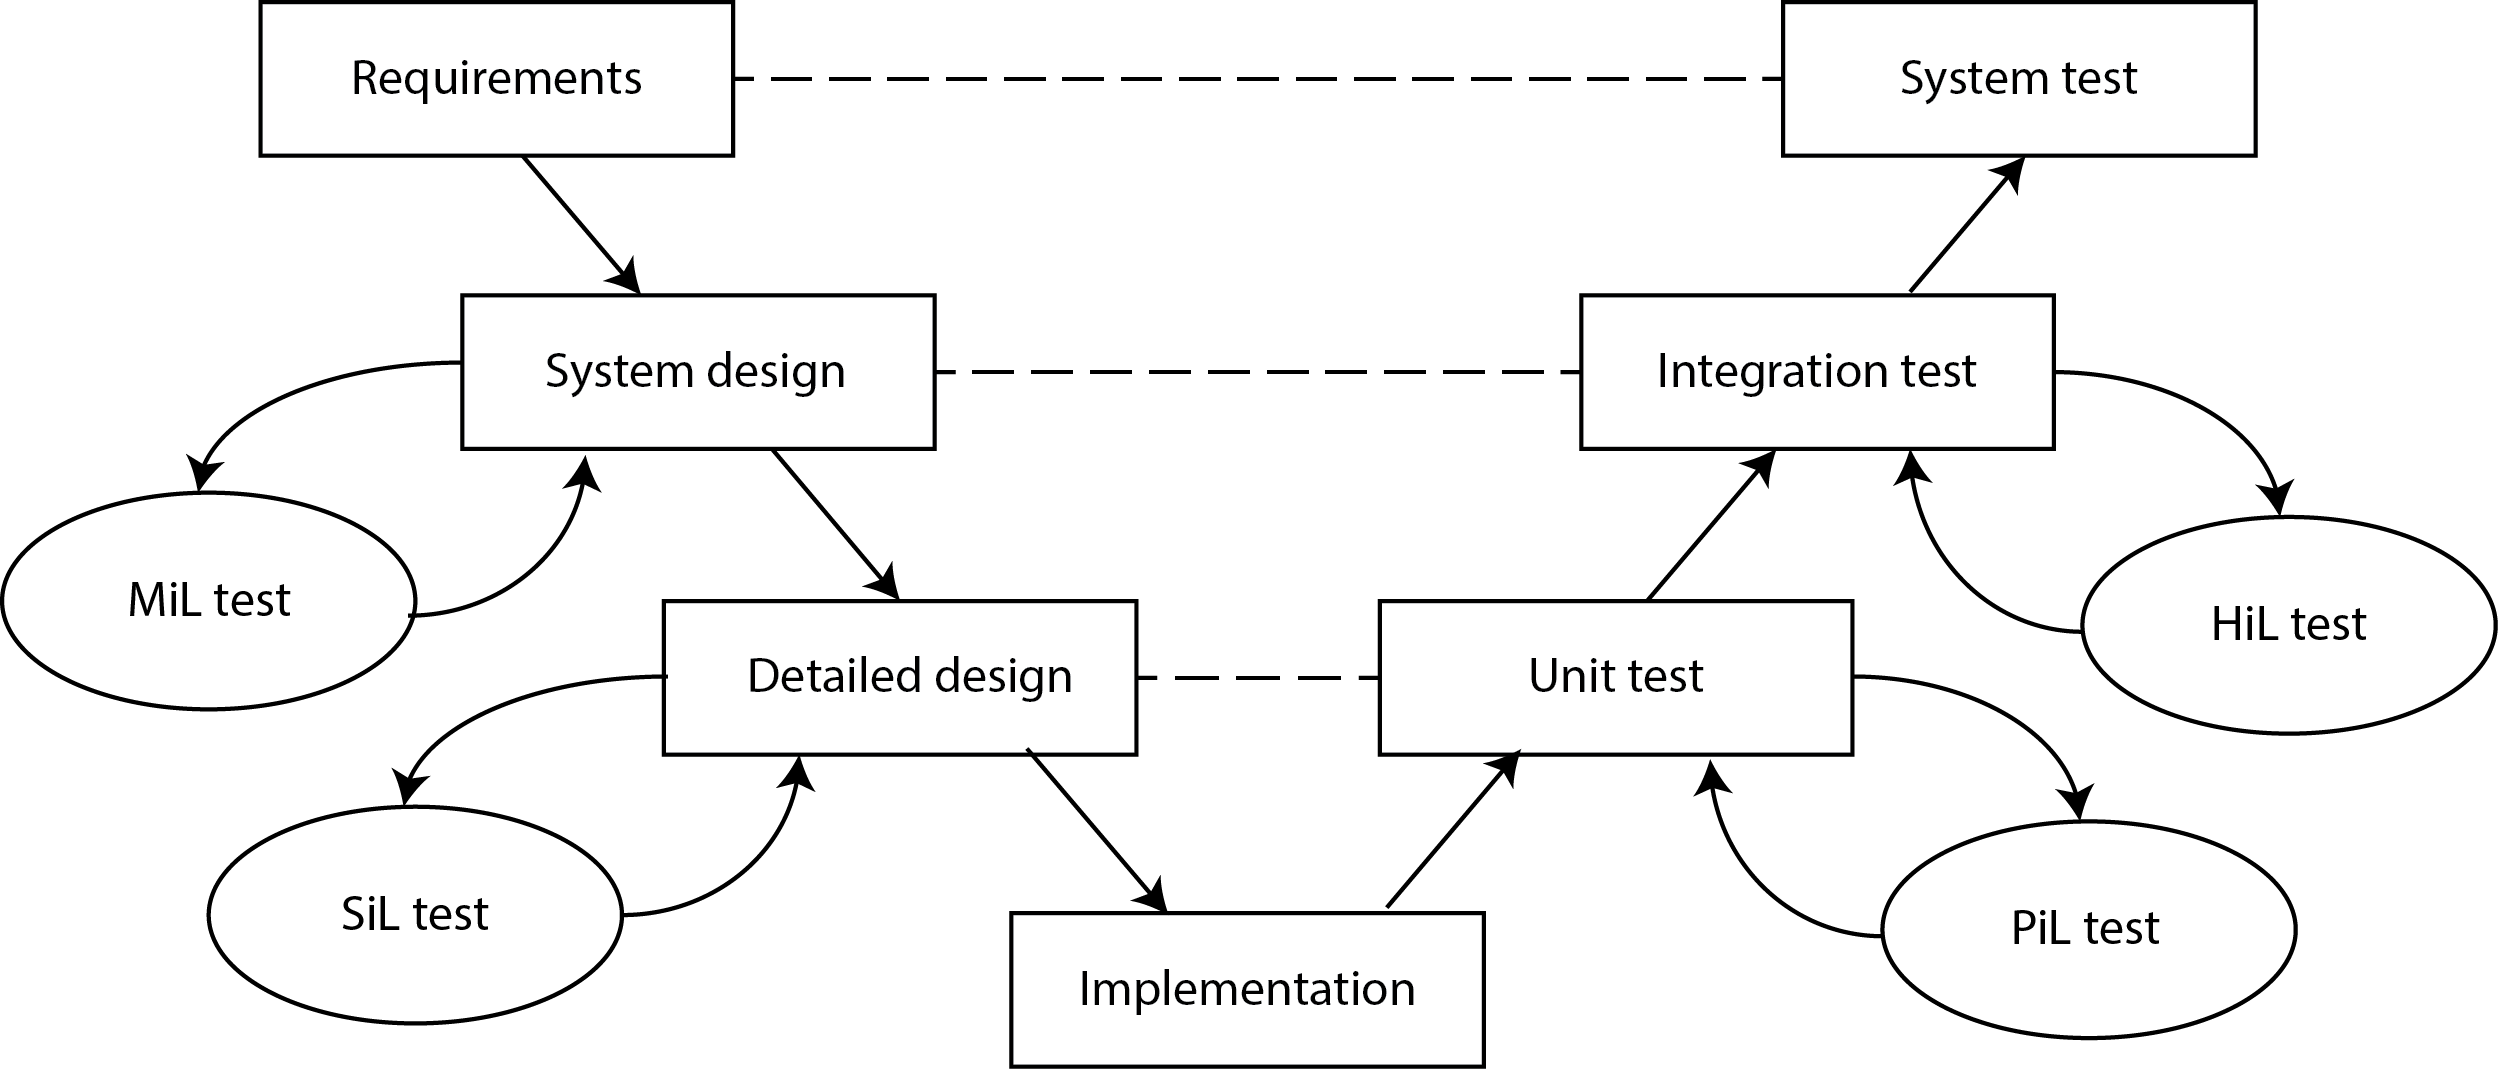
\includegraphics[width=150mm]{figures/testDesign/V_model.png}
	\caption{V-model}
	\label{fig:vModel}
\end{figure}

\subsection{V-model and testing levels}
Nowadays one of the most popular software development methodology is the V-model \cite{Vmodel} (shown on figure \ref{fig:vModel}), which defines four stages during the development and four verification steps accordingly (shown with rectangles). In addition for making the development more effective for error-detection, there are four more steps defined for verifying our system \cite{TestLevels} (shown with ellipses). While the development starts with an abstract \textbf{requirement analysis}, which declares the aim of our application, later on each step contains more detailed information. The second phase is about understanding the abstract user requirements and define the \textbf{system functional specification} by the developers. During this phase our verification is based on \textbf{Model-in-the-Loop (MiL) testing}. The third phase contains all the low-level design and specific information about the application. From these design decisions, the \textbf{implementation} should be quite straight-forward or even generated. To make sure that the code is working correctly it is tested using \textbf{Software-in-the-Loop (SiL)}. 
As of now our application code is written and our design decisions are verified, we make sure with \textbf{unit tests} that our functions are working well on their own. \textbf{Processor-in-the-Loop (PiL)} testing can be made here. Moving up in the V-model with \textbf{integration tests}, we are focusing on more abstract and complex components. In this phase we consider software and hardware elements also, completed with \textbf{Hardware-in-the-Loop (HiL)} testing. The last step is about verifying the complete system in real environment and check the high-level criterias.

\subsection{Test techniques}
\todo[inline]{give details}


\section{Test documentation}
\todo[inline]{Mention here the ISO 29119-3 with figure.}
First we should see what documents will be used in the MODES\^3 test documentation process. In the following section I will describe the used documentation from ISO 29119-3 standard. As of now the organizational and role details are irrelevant for this project, I will just give a short example for those.

\begin{figure}[!h]
	\centering
	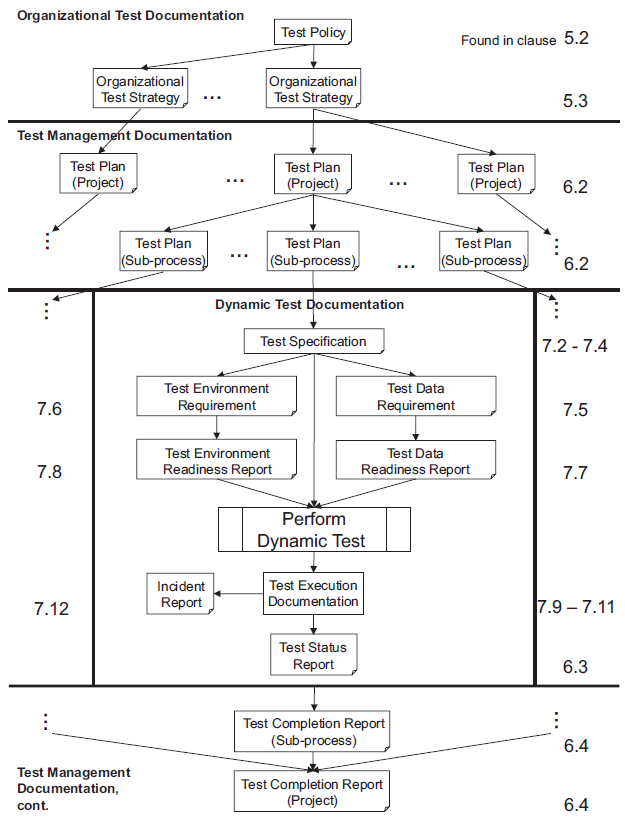
\includegraphics[width=150mm, keepaspectratio]{figures/testDesign/TestDoc.png}
	\caption{test Documentation Overview}
	\label{fig:TestDocOverview}
\end{figure}

\subsection{Organizational test documentation}
These documents should be distributed organizational-wise and should be the same for every project. In according to this, the organization will be now the MoDeS$^3$ team and the only project will be the above detailed railway system.

\paragraph{Test Policy}
In general a Test Policy must contain the test principles and objectives for the organization It clarifies what should be tested in that development phase, but not how testing must be implemented. Furthermore it must define the provisions to be used for establishing, improving, maintaining and reviewing the test Policy.

\paragraph{Test Strategy}
A Test Strategy must define a proper guideline on how testing should be performed for all projects in the organization. In our case one Test Strategy is sufficient, but for an organization which develop projects in different technical areas can have a Test Strategy for each area. In latter case, the organization can define separate Test sub-processes. 

\todo[inline]{Do I need more details about test sub-processes?}

%\begin{enumerate}
%	\item Organizational Test Strategy
%	\begin{enumerate}
%		\item Introduction
%		\item General test strategy statements
%		\begin{enumerate}
%			\item Generic risk management
%			\item Test selection and prioritization
%			\item Test documentation and reporting
%			\item Test automation and tools
%			\item Configuration management of test work products
%			\item Incident management
%			\item Test sub-processes
%		\end{enumerate}
%	\end{enumerate}
%\end{enumerate}

\subsection{Test Management Documentation}
The Test Management Documentation is focusing on one project's planning and test evaluation with Test Plan, Test Status Report and Test Completion Report guidelines.

\paragraph{Test Plan}
This document collects the test plan and test management processes including the re-planning decisions. A Test Plan can be applied to multiple projects or to a single project, where each Test Plan is dedicated for each test sub-process (Like system test plan, integration software test plan, sub-system test plan, or unit software test plan). In a complex structure it is advices to have a mapping tree showing the relations of the created Test Plans.

\paragraph{Test Status Report}
This is produced to summarize the progress of an ongoing test process in a given reporting period. For example in an agile project it can be created for every iteration, but it is not necessarily a written document.

\paragraph{Test Completion Report}
This can be provided for every test sub-process or for the whole project and contains a summary of the testing which was performed.

\subsection{Dynamic Test Documentation}
During the dynamic test process the following documents are provided:
\begin{itemize}
	\item Test Specification with sub-documents of:
	\begin{itemize}
		\item Test Design Specification
		\item Test Case Specification
		\item Test Procedure Specification
	\end{itemize}
	\item Test Data Requirements
	\item Test Environment Requirements
	\item Test Data Readiness Report
	\item Test Environment Readiness Report
	\item Test Execution Documentation with sub-documents of:
	\begin{itemize}
		\item Actual Result
		\item Test Results
		\item Test Execution Log
		\item Incident Report
	\end{itemize}
\end{itemize}
\todo[inline]{Figure with test docs hierarchy can be added here}

I will give a brief summary for each documentation approach.

\paragraph{Test Design Specification} \label{TestDoc:TDS}
The features and test conditions (derived from test basis) are collected in the Test Design Specification with the specific test cases and test procedures. These detailed test cases will be executed during testing process. 

Here we can create logical groups called \textit{feature sets} for those features which can be tested independently.  A \textit{test condition} is aligned for each feature set and can be independently verified by a test case and can reference a requirement (or a group of them). Take care of test condition's traceability and priority.

\paragraph{Test Case Specification}
For one or more feature set, the Test Case Specification describes a set of test cases with the corresponding test coverage items.

A set of test conditions performed with a specific test design technique creates a \textit{test coverage item}, which can be summarized in a list (showing test coverage items, test conditions and feature sets with proper priorities). From each test coverage item a \textit{Test case} can be derived, which determines the correct implementation of a test item. Regarding the possible number of test cases it can be collected into a list, table or database. 
Each test case should have a proper definition of dependencies. These are collected in \autoref{table:TestDoc:TestCases}.

\begin{table}[h]
	\caption{Details of each test case}
	\label{table:TestDoc:TestCases}
	\begin{center}
		\renewcommand{\arraystretch}{1.8}
		\begin{tabu} 
			to 0.9 \textwidth
			{  X[c]  X[c] }
			\toprule
			Aspect                          & Description                                                                                                                                               \\ \midrule
			Priority                        & Higher priority test cases should be examined earlier then lower priorities                                                                               \\
			Traceability                    & Each test case can be traceable from each requirement through test coverage items                                                                         \\
			Preconditions                   & Describes special states that must exists to execute the test case (Can be other test cases also)                                                         \\
			Inputs                          & A specific action which sets the test item into a state, where the actual and expected results can be compared                                            \\
			Expected results                & Specifies the expected output and behavior (with tolerances) of the test item which was in the precondition state and was modified with the proper inputs \\
			Actual results and test results & A description of test item outputs and the comparison to expected results                                                                                 \\ \bottomrule
		\end{tabu}
	\end{center}
\end{table} 

\paragraph{Test Procedure Specification}
Describes the precondition setup and test cases execution in the proper order, with possible post evaluation activities.

\textit{Test sets} can be collected for those test cases, which have the same purpose regarding test item, precondition, test basis or even by the identified risk. Typically this will reflect to one or more feature sets. For each \textit{Test set} the proper execution order is defined in the \textit{Test procedure} according to test case dependencies, preconditions, postconditions and other environment requirements.

\paragraph{Test Data Requirements}
Defines the required properties of test data, which is used during test procedure execution. It can be collected into a list detailed test data requirements, making it maintainable and trackable. 

\paragraph{Test Data Readiness Report} 
Gives a list of Test Data Requirements if they are satisfied or not with a proper authorization.

\paragraph{Test Environment Requirements}
Describes the required test environment properties, setting the test items into the desired test environment to be able to execute test procedures. These requirements can also be grouped by environment types like hardware, middleware, software, tools or security.

\paragraph{Test Environment Readiness Report}
Describes the fulfillment of Test Environment Requirements.

\paragraph{Actual Results}
After executing the selected test procedures, each test case's actual result (output state or behavior) should be recorded. It may require full recording of the process with an automated tool also.

\paragraph{Test Result}
Determines if the actual result is correspond to the expected results with the specified deviation or not. It is usually recorded as passed or failed, along with the actual results.

\paragraph{Test Execution Log}
Detailed documentation of one or more test procedure's execution. Can be described in a list or table with measured times and event of the test execution.

\paragraph{Test Incident Reporting}
At the end of the test execution for failed test cases and findings we can create dedicated Incident Reports. These reports could contain the incident description itself with severity, date and possible risk information.


\section{Test Documentation for MoDeS$^3$ project}
\todo[inline]{Wat about: test process, organization test evaluation, test improvement sections?}

\subsection{Test Policy for MoDeS$^3$ organization}
\paragraph{Scope:} This Test Policy will be followed by the MoDeS$^3$ team in the Department of Measurement and Information Systems, which will provide us a testing framework for the railway system project.
\paragraph{Introduction:} The railway system project have started several years back, and from time to time the team faced smaller and bigger problems with the implementation. Approximately a lot of them could be prevented with a details test documentations and process. To avoid these situations in the future I will now introduce a test documentation approach.
\paragraph{Objectives of testing:} The objective of testing is to measure and improve the software quality and to avoid safety-critical failures in the system.
\paragraph{Standards:} The testing documentation will follow the ISO/IEC/IEEE standard 291119-3 "Test Documentation".

\subsection{Test Strategy for MoDeS$^3$ projects}
\paragraph{Scope:} The following test strategy is applicable for the railway system project. This strategy's aim is to support testing in the software development phases in component and system level also.
\paragraph{Risk management:} For each specific test plan the risk management must be handled separately. The detailed format must be a traceable list or table. 
\paragraph{Test selection prioritization:} The test cases and test procedures will follow a bottom-up strategy priorization aligned with safety-critical risk levels. Consequently a test element with lower dependencies and more independent functionality got higher priority then a complex test element, which rely on multiple sub components. 
\paragraph{Test document and reporting:} The test process and documentation must be well-separated and clear that a new team member can easily understand the structure.
\paragraph{Test automation and tools:} All tools, which is used during the test process and documentation must be available for a university student (with education license or freely).
\paragraph{Incident management:} All detected defects must be created as a github issue also.
%\paragraph{Test sub-processes:} All test projects must provide the following test levels: unit test, integration test, system test.
\todo[inline]{strategy todo: scope? risk management? github clarification, test sub-processes?}

\subsection{Test Completion Report}
\todo[inline]{fill out in connection with progress}

\subsection{Master Test Plan for Railway System project}\label{section:MTP}
\paragraph{Scope:} Test plan's scope is to provide the necessary test framework for testing the railway system of MoDeS$^3$ team. This document identifies a way for planning, executing and maintaining tests in a multi-layered project.
\paragraph{Plan context:} The railway system architecture (detailed in \autoref{chapter:RailwaySystem}) consist of off-the-shelf products, custom hardware and software elements. According to this, the \textit{test items} are only the custom software elements, which were made by the MoDeS$^3$ team. Details about test items can be found in \autoref{section:CustomSW}. The standard product's testing and the hardware extension's verifications are not part of the Test Plan.
\paragraph{Risk register:}
For a railway system the possible safety-critical aspects are detailed in \autoref{section:SC-Functionalities}.
\todo[inline]{Create metrics for the risk table}
\begin{table}[h]
\caption{Project risks}
\label{table:Risks-Safety-critical}
	\begin{center}
		\renewcommand{\arraystretch}{1.8}
		\begin{tabu} 
			to 0.9 \textwidth
			{ X[l] X[l] }
			\toprule
			Risk ID                                                                                     & Mitigation activities                                                                 \\ \midrule
			%			                                            \multicolumn{2}{c}{Occupancy detection}     &  \\
			1 Wrong or no occupancy detected                                                            & Review of design and appropriate hardware and software elements .                     \\
			%			                                         \multicolumn{2}{c}{Track element controlling}  &  \\
			2 Not controllable turnout  or segment                                                      & Review of hardware and software components.                                            \\
			%			                                       \multicolumn{2}{c}{Safety critical verification} &  \\
			3 Wrong collision avoidance decision made                                                   & Review of design and safety algorithm. Extra test cases to cover additional scenarios. \\
			4 Train collision                                                                           & Review of design and safety algorithm.                                                \\ \bottomrule
		\end{tabu}
	\end{center}
\end{table} 
\paragraph{Test strategy:} 
We define \textit{test sub-processes} for the railway system project:
\begin{itemize}
	\item Unit test
	\item Integration test
	\item System test
\end{itemize}
In addition for all sub-processes the following documents must be delivered:
\begin{itemize}
	\item Test sub-process plan
	\item Test specification
	\item Test log
	\item Test sub-process completion report
\end{itemize}
The test design techniques, test completion criteria and test data must apply to every test sub-process. We use the following test environments in general:
\begin{itemize}
	\item Eclipse Photon where applicable
	\item Visual Studio Code where applicable
	\item Xtend 
	\item JUnit Jupiter for Java base components
	\item Mockito with PowerMockito for Java base components
	\item GTest for C++ components
	\item Railway track elements
\end{itemize}
\paragraph{Test activities and estimates:} These are confirmed personally with university studies.
\paragraph{Stuffing:} The actual team and roles are highly dependent in the MoDeS$^3$ team in every semester.
\paragraph{Retesting and regression testing:} This is specified for each test sub-process.
\todo[inline]{Verify Test envs? sub processes? risk man.? }


\subsection{Unit Test Plan}
\paragraph{Scope:} See the \autoref{section:MTP} for Master Test Plan. The aim for this Test Plan is to verify each software component's functionality independently.
\paragraph{Plan context:} Unit Test Plan context is the same as for Master Test Plan (see \autoref{section:MTP}), because all self developed software component must be tested in a standalone environment. 
\paragraph{Risk register:}
\paragraph{Test strategy:} The deliverables are this test plan, the test specification for unit test and the test completion report. 
During the test process and documentation the decision coverage and fault attack test design techniques are relevant.
Each unit must reach a 80\%  requirement coverage. 
%\paragraph{Test activities and estimates:}

\todo[inline]{Risks? link the test deliverables, complete test design techniques, test activities?}

\subsection{Integration Test Plan}

\subsection{System Test Plan}







\subsection{Test Design Specification for Unit Test Plan}

\paragraph{Purpose:} The purpose of this test specification is to give a guideline for executing unit tests.
\paragraph{References:} The railway system related requirements can be found in \autoref{section:REQ}.

\subsubsection{Feature Sets} We can easily separate the system's functionalities into feature sets following the referenced system requirement's structure. The \autoref{table:Feature-Sets} are containing the feature sets.
\begin{table}[!h]
\caption{Feature sets}
\label{table:Feature-Sets}
	\begin{center}
		\renewcommand{\arraystretch}{1.8}
		\begin{tabu} 
			to 1.0 \textwidth
			{  X[0.7,c] X[1.5, c] X[3.0, c] X[0.7,c] X[c] X[2.0,c] }
			\toprule
			\multicolumn{2}{c}{Feature Set} & Scope                                                                                            & Priority & Approach & Traceability                                                                   \\ \midrule
			ID   & Name                     &                                                                                                  &          &          &                                                                                \\ \midrule
			FS-1 & TO BE DELETED: Train detection          & To test train measurement functionalities                                                        & TODO     &          & \ref{req:TD}                                                                   \\
			FS-2 & GPIO handling            & To test GPIO pin handling                                                                        & TODO     &          & \ref{req:GPIO}                                                                 \\
			FS-3 & Occupancy detection      & To test the occupancy related functionalities in the system including state and change detection & TODO     &          & \ref{req:OCQ-1}, \ref{req:OCQ-2}, \ref{req:SOQ}                                \\
			FS-4 & Track element controller & To test segment's availability and turnout's direction setting                                   & TODO     &          & \ref{req:TEC-1}, \ref{req:TEC-2}                                               \\
			FS-5 & Safety Logic             & To test railway system's safety logic                                                            & TODO     &          & \ref{req:SL-1}, \ref{req:SL-2} , \ref{req:SL-3}, \ref{req:SL-4}                \\
			FS-6 & Dashboard                & To test Dashboard's capabilities                                                                 & TODO     &          & \ref{req:DB-1}, \ref{req:DB-2}, \ref{req:DB-3}, \ref{req:DB-4}, \ref{req:DB-5} \\ \bottomrule
		\end{tabu}
	\end{center}
\end{table} 

\subsubsection{Test Conditions} In the following section I will describe the test conditions for each feature set. In this test plan, most of the feature sets are simple functions, consequently the test conditions also will describe the test coverage items.
\paragraph{TO BE DELETED: Train detection (FS-1)}
\todo[inline]{Verify speeds, length range}
\begin{table}[!h]
\caption{Train detection test conditions}
\label{table:TC-FS-1}
	\begin{center}
		\renewcommand{\arraystretch}{1.8}
		\begin{tabu} 
			to 0.9 \textwidth
			{  X[c] X[c] X[c] X[c] }
			\toprule
			Test condition & Measuring type & Value  & Comment                  \\ \midrule
			FS-1/1.0       & Speed          & 0 km/h & Standing train           \\
			FS-1/1.1       & Speed          & 1 km/h & Train with average speed \\
			FS-1/1.2       & Speed          & 5 km/h & Train with max speed     \\
			FS-1/2.0       & Length         & 15cm   & Average length           \\ \bottomrule
		\end{tabu}
	\end{center}
\end{table} 

\paragraph{GPIO handling (FS-2)}
Considering the GPIO's functionality the following test conditions are test coverage items also (see \autoref{table:TC-FS-2}).
\begin{table}[!h]
	\caption{GPIO handling test condition}
	\label{table:TC-FS-2}
	\begin{center}
		\renewcommand{\arraystretch}{1.8}
		\begin{tabu} 
			to 0.9 \textwidth
			{  X[c] X[c] X[c] X[c] X[c] }
			\toprule
			Test condition & Direction                     & Phase                            & Configuration file           & Setting \\ \midrule
			FS-2/1.0       & \centeredDoubleRow{3}{Input}  & Initialization                   & edge                         & BOTH    \\
			FS-2/1.1       &                               & \centeredDoubleRow{2}{Operation} & \centeredDoubleRow{2}{value} & LOW     \\
			FS-2/1.2       &                               &                                  &                              & HIGH    \\
			FS-2/2.0       & \centeredDoubleRow{2}{Output} & Initialization                   & \centeredDoubleRow{3}{value} & LOW     \\
			FS-2/2.1       &                               & \centeredDoubleRow{2}{Operation} &                              & LOW    \\
			FS-2/2.2       &                               &                                  &                              & HIGH     \\ \bottomrule
		\end{tabu}
	\end{center}
\end{table} 

\paragraph{Occupancy detection (FS-3)}
Because of the component's simplicity there are 2 test condition items and also considered as test coverage items (items are shown in \autoref{table:TC-FS-3}). The values are observed as the periodic occupancy detection result for one section.
\begin{table}[!h]
	\caption{Occupancy detection test condition and coverage items}
	\label{table:TC-FS-3}
	\begin{center}
		\renewcommand{\arraystretch}{1.8}
		\begin{tabu} 
			to 0.9 \textwidth
			{  X[c] X[c] X[c] }
			\toprule
			Test condition & Value    & Comment             \\ \midrule
			FS-3/1.0       & Free     & Specific segment is free     \\
			FS-3/1.1       & Occupied & Specific segment is occupied \\ \bottomrule
		\end{tabu}
	\end{center}
\end{table}


\paragraph{Track element controller (FS-4)}
A track element controller can handle segment and turnout section types also, consequently we distinguish these types with the possible states for the definition of test condition and coverage item. (Shown in \autoref{table:TC-FS-4}.)
\begin{table}[!h]
	\caption{Track element controller test condition and coverage items}
	\label{table:TC-FS-4}
	\begin{center}
		\renewcommand{\arraystretch}{1.8}
		\begin{tabu} 
			to 0.9 \textwidth
			{  X[c] X[c] X[c] }
			\toprule
			Test condition & Affected element               & Enabled     \\ \midrule
			FS-4/1.0       & \centeredDoubleRow{2}{Segment} & Disabled   \\
			FS-4/1.1       &                                & Occupied  \\
			FS-4/2.0       & \centeredDoubleRow{2}{Turnout} & Straight  \\
			FS-4/2.1       &                                & Divergent \\ \bottomrule
		\end{tabu}
	\end{center}
\end{table} 

\paragraph{Safety Logic (FS-5)}
The safety-critical aspects are shown in \autoref{table:TC-FS-5}, which should be prevented by the Safety Logic.
\begin{table}[!h]
	\caption{Safety Logic test condition}
	\label{table:TC-FS-5}
	\begin{center}
		\renewcommand{\arraystretch}{1.8}
		\begin{tabu} 
			to 0.9 \textwidth
			{  X[c] X[c] X[c] }
			\toprule
			Test condition & Safety Level                  & Safety type     \\ \midrule
			FS-5/1.0       & \centeredDoubleRow{2}{System} & Train collision \\
			FS-5/2.0       &                               & Turnout derail  \\ \bottomrule
		\end{tabu}
	\end{center}
\end{table} 

\paragraph{Dashboard (FS-6)}
A full functional coverage is aimed for the Dashboard which can be defined by the following test condition and coverage items shown in \autoref{table:TC-FS-6}.
\begin{table}[!h]
	\caption{Dashboard test conditions}
	\label{table:TC-FS-6}
	\begin{center}
		\renewcommand{\arraystretch}{1.8}
		\begin{tabu} 
			to 0.9 \textwidth
			{  X[c] X[c] X[c] X[c] }
			\toprule
			Test condition & Affection                   & Section type                   & State     \\ \midrule
			FS-6/1.0       & \centeredDoubleRow{4}{All}  & \centeredDoubleRow{2}{Turnout} & Straight  \\
			FS-6/1.1       &                             &                                & Divergent \\
			FS-6/1.2       &                             & \centeredDoubleRow{2}{Segment} & Enabled   \\
			FS-6/1.3       &                             &                                & Disabled  \\
			FS-6/2.0       & \centeredDoubleRow{4}{Each} & \centeredDoubleRow{2}{Turnout} & Straight  \\
			FS-6/2.1       &                             &                                & Divergent \\
			FS-6/2.2       &                             & \centeredDoubleRow{2}{Segment} & Enabled   \\
			FS-6/2.3       &                             &                                & Disabled  \\ \bottomrule
		\end{tabu}
	\end{center}
\end{table} 


\subsubsection{Test coverage items}
\todo[inline]{diagrams for each test coverage item}
\paragraph{Safety Logic: Train collision test coverage items (FS-5/1.0)}
\begin{enumerate}[label=FS-5/1.0-\arabic*, leftmargin=*, format=\small]
	\item 1 Train is moving to a segment where there is an other train
	\item 1 Train is moving to a segment where the other train is 1 distance away on the path
	\item 1 Train is moving to a segment where the other train is 2 distance away on the path
\end{enumerate}
\paragraph{Safety Logic: Turnout derail test coverage items (FS-5/2.0)}
\begin{enumerate}[label=FS-5/2.0-\arabic*, leftmargin=*, format=\small]
	\item Train is moving through a turnout from top to divergent, while the turnout is in straight state
	\item Train is moving through a turnout from top to straight, while the turnout is in divergent state
\end{enumerate}

\subsubsection{Test cases}\label{section:UnitTestCases}
In this section I will describe the test cases defined by test conditions and coverage items for each feature set.
\paragraph{Gpio Handling (FS-2)} In order to work in production with GPIO component, the following configuration file must exists: sys/gpio/gpioPIN/export, sys/gpio/gpioPIN/value and sys/gpio/gpioPIN/edge. This need is also propagate to all test cases regarding GPIO handling, so files are created or mocked.
\todo[inline]{priority}
\begin{table}[H]
	\caption{Test case 2-1}
	\label{table:TCase-FS2-1}
	\begin{center}
		\renewcommand{\arraystretch}{1.8}
		\begin{tabu} 
			to 0.9 \textwidth
			{  X[0.4, c] X[c] }
			\toprule
			Test case ID: 2-1 \newline Priority: am \newline Tracing: FS-2/1.0 & Purpose: to test the GPIO initialization in input direction       \\ \midrule
			Precondition                                                       & The GPIO's necessary files are available                          \\
			Input                                                              & Initialize the GPIO itself with input direction.                  \\
			Expected result                                                    & The "both" string have been written to "edge" configuration file. \\ \bottomrule
		\end{tabu}
	\end{center}
\end{table} 

\begin{table}[!h]
	\caption{Test case 2-2}
	\label{table:TCase-FS2-2}
	\begin{center}
		\renewcommand{\arraystretch}{1.8}
		\begin{tabu} 
			to 0.9 \textwidth
			{  X[0.4, c] X[c] }
			\toprule
			Test case ID: 2-2 \newline Priority: am \newline Tracing: FS-2/1.1 & Purpose: to test the GPIO pin change listener while direction is input, value is "0"  \\ \midrule
			Precondition                                                       & The GPIO's necessary files are available                                              \\
			Input                                                              & The value file have been written to "0" considered as LOW.                            \\
			Expected result                                                    & GPIO noticed the change and read the "value" configuration file content as LOW level. \\ \bottomrule
		\end{tabu}
	\end{center}
\end{table} 

\begin{table}[H]
	\caption{Test case 2-3}
	\label{table:TCase-FS2-3}
	\begin{center}
		\renewcommand{\arraystretch}{1.8}
		\begin{tabu} 
			to 0.9 \textwidth
			{  X[0.4, c] X[c] }
			\toprule
			Test case ID: 2-3 \newline Priority: am \newline Tracing: FS-2/1.2 & Purpose: to test the GPIO pin change listener while direction is input, value is "1"   \\ \midrule
			Precondition                                                       & The GPIO's necessary files are available                                               \\
			Input                                                              & The value file have been written to "1" considered as HIGH.                            \\
			Expected result                                                    & GPIO noticed the change and read the "value" configuration file content as HIGH level. \\ \bottomrule
		\end{tabu}
	\end{center}
\end{table} 

\begin{table}[H]
	\caption{Test case 2-4}
	\label{table:TCase-FS2-4}
	\begin{center}
		\renewcommand{\arraystretch}{1.8}
		\begin{tabu} 
			to 0.9 \textwidth
			{  X[0.4, c] X[c] }
			\toprule
			Test case ID: 2-4 \newline Priority: am \newline Tracing: FS-2/2.0 & Purpose: to test the GPIO initialization in output direction.   \\ \midrule
			Precondition                                                       & The GPIO's necessary files are available                        \\
			Input                                                              & Initialize the GPIO itself with output direction.               \\
			Expected result                                                    & The "0" string have been written to "value" configuration file. \\ \bottomrule
		\end{tabu}
	\end{center}
\end{table} 

\begin{table}[H]
	\caption{Test case 2-5}
	\label{table:TCase-FS2-5}
	\begin{center}
		\renewcommand{\arraystretch}{1.8}
		\begin{tabu} 
			to 0.9 \textwidth
			{  X[0.4, c] X[c] }
			\toprule
			Test case ID: 2-5\newline Priority: am \newline Tracing: FS-2/2.1 & Purpose: to test the GPIO pin's level setting to LOW \\ \midrule
			Precondition                                                      & The GPIO's necessary files are available             \\
			Input                                                             & Set the GPIO's level to LOW.                         \\
			Expected result                                                   & The "value" file has been modified with value "0"    \\ \bottomrule
		\end{tabu}
	\end{center}
\end{table} 

\begin{table}[H]
	\caption{Test case 2-6}
	\label{table:TCase-FS2-6}
	\begin{center}
		\renewcommand{\arraystretch}{1.8}
		\begin{tabu} 
			to 0.9 \textwidth
			{  X[0.4, c] X[c] }
			\toprule
			Test case ID: 2-6 \newline Priority: am \newline Tracing: FS-2/2.2 & Purpose: to test the GPIO pin's level setting to HIGH \\ \midrule
			Precondition                                                       & The GPIO's necessary files are available              \\
			Input                                                              & Set the GPIO's level to HIGH.                         \\
			Expected result                                                    & The "value" file has been modified with value "1"     \\ \bottomrule
		\end{tabu}
	\end{center}
\end{table} 

\paragraph{Occupancy detection (FS-3)}
\begin{table}[H]
	\caption{Test case 3-1}
	\label{table:TCase-FS3-1}
	\begin{center}
		\renewcommand{\arraystretch}{1.8}
		\begin{tabu} 
			to 0.9 \textwidth
			{  X[0.4, c] X[c] }
			\toprule
			Test case ID: 3-1 & Purpose: to test detection of occupancy components, when the specific segment is free\newline Priority: above middle \newline Tracing: (FS-3/1.0)\\ \midrule
			Precondition & S88 serial port connection  \\
			Input & Unclosed circuit between the specific segment's hardware elements  \\
			Expected result & Occupancy components have queried free occupancy state \\ \bottomrule
		\end{tabu}
	\end{center}
\end{table} 

\begin{table}[H]
	\caption{Test case 3-2}
	\label{table:TCase-FS3-2}
	\begin{center}
		\renewcommand{\arraystretch}{1.8}
		\begin{tabu} 
			to 0.9 \textwidth
			{  X[0.4, c] X[c] }
			\toprule
			Test case ID: 3-1 & Purpose: to test detection of occupancy components, when the specific segment is occupied \newline Priority: above middle \newline Tracing: (FS-3/1.1)\\ \midrule
			Precondition & S88 serial port connection  \\
			Input & Closed circuit between the specific segment's hardware elements  \\
			Expected result & Occupancy components have queried occupied occupancy state \\ \bottomrule
		\end{tabu}
	\end{center}
\end{table} 

\paragraph{Track element controller (FS-4)}
\begin{table}[H]
	\caption{Test case 4-1}
	\label{table:TCase-FS4-1}
	\begin{center}
		\renewcommand{\arraystretch}{1.8}
		\begin{tabu} 
			to 0.9 \textwidth
			{  X[0.4, c] X[c] }
			\toprule
			Test case ID: 4-1 & Purpose: to test the track element controller's segment state setting as enabled \newline Priority: above middle \newline Tracing: (FS-4/1.0)\\ \midrule
			Precondition & Observable GPIO components \\
			Input & Call the track element controller set segment state function with enabled parameter  \\
			Expected result & All GPIO's levels are in "HIGH" state, which are related to the specific segment \\ \bottomrule
		\end{tabu}
	\end{center}
\end{table}

\begin{table}[H]
	\caption{Test case 4-2}
	\label{table:TCase-FS4-2}
	\begin{center}
		\renewcommand{\arraystretch}{1.8}
		\begin{tabu} 
			to 0.9 \textwidth
			{  X[0.4, c] X[c] }
			\toprule
			Test case ID: 4-2 & Purpose: to test the track element controller's segment state setting as disabled\newline Priority: above middle \newline Tracing: (FS-4/1.1)\\ \midrule
			Precondition & Observable GPIO components \\
			Input & Call the track element controller set segment state function with disabled parameter  \\
			Expected result & All GPIO's levels are in "LOW" state, which are related to the specific segment \\ \bottomrule
		\end{tabu}
	\end{center}
\end{table} 

\begin{table}[H]
	\caption{Test case 4-3}
	\label{table:TCase-FS4-3}
	\begin{center}
		\renewcommand{\arraystretch}{1.8}
		\begin{tabu} 
			to 0.9 \textwidth
			{  X[0.4, c] X[c] }
			\toprule
			Test case ID: 4-3 & Purpose: to test the track element controller's turnout changing to straight state\newline Priority: above middle \newline Tracing: (FS-4/2.0)\\ \midrule
			Precondition & Observable GPIO components \\
			Input & Call the track element controller set turnout state function with straight parameter  \\
			Expected result & The GPIO, which is controlling the straight branch, sending an impulse sign (inverting the current level twice with a specific time shift) \\ \bottomrule
		\end{tabu}
	\end{center}
\end{table}

\begin{table}[H]
	\caption{Test case 4-4}
	\label{table:TCase-FS4-4}
	\begin{center}
		\renewcommand{\arraystretch}{1.8}
		\begin{tabu} 
			to 0.9 \textwidth
			{  X[0.4, c] X[c] }
			\toprule
			Test case ID: 4-4 & Purpose: to test the track element controller's turnout changing to divergent state\newline Priority: above middle \newline Tracing: (FS-4/2.1)\\ \midrule
			Precondition & Observable GPIO components \\
			Input & Call the track element controller set turnout state function with divergent parameter  \\
			Expected result & The GPIO, which is controlling the divergent branch, sending an impulse sign (inverting the current level twice with a specific time shift) \\ \bottomrule
		\end{tabu}
	\end{center}
\end{table}

\paragraph{Safety logic (FS-5)}
\begin{table}[H]
	\caption{Test case 5-1}
	\label{table:TCase-FS5-1}
	\begin{center}
		\renewcommand{\arraystretch}{1.8}
		\begin{tabu} 
			to 0.9 \textwidth
			{  X[0.4, c] X[c] }
			\toprule
			Test case ID: 5-1 & Purpose: to test the safety logic awareness, when a train is moving on a path where the next section in the direction already occupied by a train \newline Priority: high \newline Tracing: (FS-5/1.0)\\ \midrule
			Precondition & None  \\
			Input & Insert a train to a specific segment and move an other train to the adjacent segment\\
			Expected result & Safety Logic sent a segment disable command with the id of the specific segment \\ \bottomrule
		\end{tabu}
	\end{center}
\end{table} 


\begin{table}[H]
	\caption{Test case 5-2}
	\label{table:TCase-FS5-2}
	\begin{center}
		\renewcommand{\arraystretch}{1.8}
		\begin{tabu} 
			to 0.9 \textwidth
			{  X[0.4, c] X[c] }
			\toprule
			Test case ID: 5-2 & Purpose: to test the safety logic awareness, when a train is moving and in the 2nd section in the path is already occupied by a train \newline Priority: high \newline Tracing: (FS-5/1.0-1)\\ \midrule
			Precondition & None  \\
			Input & Insert a train to a specific segment and move an other train there from a 2 distance away segment\\
			Expected result & Safety Logic sent a segment disable command with the id of the specific segment \\ \bottomrule
		\end{tabu}
	\end{center}
\end{table} 

\begin{table}[H]
	\caption{Test case 5-3}
	\label{table:TCase-FS5-3}
	\begin{center}
		\renewcommand{\arraystretch}{1.8}
		\begin{tabu} 
			to 0.9 \textwidth
			{  X[0.4, c] X[c] }
			\toprule
			Test case ID: 5-2 & Purpose: to test the safety logic awareness, when a train is moving and in the 3rd section in the path is already occupied by a train \newline Priority: high \newline Tracing: (FS-5/1.0-2)\\ \midrule
			Precondition & None  \\
			Input & Insert a train to a specific segment and move an other train there from a 3 distance away segment\\
			Expected result & Safety Logic sent a segment disable command with the id of the specific segment \\ \bottomrule
		\end{tabu}
	\end{center}
\end{table} 

\begin{table}[H]
	\caption{Test case 5-4}
	\label{table:TCase-FS5-4}
	\begin{center}
		\renewcommand{\arraystretch}{1.8}
		\begin{tabu} 
			to 0.9 \textwidth
			{  X[0.4, c] X[c] }
			\toprule
			Test case ID: 5-4 & Purpose: to test the safety logic awareness, when a train is going through a turnout from top to straight, but the turnout is in divergent state \newline Priority: high \newline Tracing: (FS-5/2.0-1)\\ \midrule
			Precondition & Set the specific turnout into divergent state  \\
			Input & Set a train to go through the specific turnout from top branch to straight branch \\
			Expected result & Safety Logic sent a turnout disable command with the id of the specific turnout \\ \bottomrule
		\end{tabu}
	\end{center}
\end{table} 



\begin{table}[H]
	\caption{Test case 5-5}
	\label{table:TCase-FS5-5}
	\begin{center}
		\renewcommand{\arraystretch}{1.8}
		\begin{tabu} 
			to 0.9 \textwidth
			{  X[0.4, c] X[c] }
			\toprule
			Test case ID: 5-5 & Purpose: to test the safety logic awareness, when a train is going through a turnout from top to divergent, but the turnout is in straight state \newline Priority: high \newline Tracing: (FS-5/2.0-2)\\ \midrule
			Precondition & Set the specific turnout into straight state  \\
			Input & Set a train to go through the specific turnout from top branch to divergent branch \\
			Expected result & Safety Logic sent a turnout disable command with the id of the specific turnout \\ \bottomrule
		\end{tabu}
	\end{center}
\end{table} 



\noindent\subsubsection{Test Procedure Specification}
In this unit scoped test plan, each feature set is derived from software components in the railway system. Regarding this property each test set can involve a group of test cases which are related for one feature set. A unit test must be a fast, isolated, repeatable, self-validating execution. Because of the that test set's ordering should not influence the test results. Consequently we can consider an order as the test cases ordered in the Test case definition section (described in \autoref{section:UnitTestCases}) and one test procedure can contain one test set. 
\todo[inline]{Create tables for 5 test procedures, which lists the test cases grouped by components?}


\subsection{Test Status Report}
\todo[inline]{fill out in connection with progress}



%
%\section{Test scenarios for MoDeS$^3$}
%In the following section I will investigate the test opportunities for the MoDeS$^3$ system.  The \ref{table:test_cases} table shows the software components for different test levels and layouts. In the table a check mark shows the possibility to test that component in that exact level/layout. For the other cases testing is irrelevant. I have defined four integration test layouts, and for each test layout a component is involved where a check mark is shown. All the software components, which is deployed to other hardware components have network communication, therefore the messenger software component is also involved in that test.
%
%\subsection{Unit test}
%Those components in the system which have some logic or crucial functional responsibility, should have been verified separately also. Furthermore not all the software component have been mentioned on the \ref{table:test_cases} table, because not safety critical or purely hardware components have been skipped. \textit{Barrier} is irrelevant regarding the train-collision detection. How the trains get speed and direction controls is not safety critical either, so \textit{LeapMotion} and \textit{XPressNet} components are not safety critical. \textit{Touchboard} and \textit{Dashboard} components are only visualizing the railway current states send commands to the system, so these are not relevant elements in terms of train collision.
%
%\begin{table}[h]
%	\caption{Component test possibilities in test levels}
%	\label{table:test_cases}
%	\begin{center}
%		\renewcommand{\arraystretch}{1.8}
%		\begin{tabu} 
%			to 0.9 \textwidth
%			 {  m{4.5 cm}  c  X[c] X[c] X[c] X[c]  X[c]  }
%			\toprule
%			\centeredDoubleRow{2}{Component Name} & \centeredDoubleRow{2}{Component} &          \multicolumn{4}{c}{Integration}          & System     \\
%			\cmidrule(rl){3-6} \cmidrule(l){7-7}  &                                  & layout 1   & layout 2   & layout 3   & layout 4   & layout 1   \\ \midrule
%			Section Occupancy Query               & \checkmark                       & \checkmark &            & \checkmark &            & \checkmark \\
%			Occupancy Query                       & \checkmark                       & \checkmark &            & \checkmark &            & \checkmark \\
%			GPIO                                  & \checkmark                       &            & \checkmark &            & \checkmark & \checkmark \\
%			Track Element Controller              & \checkmark                       &            & \checkmark &            & \checkmark & \checkmark \\
%			Safety Logic                          & \checkmark                       &            &            & \checkmark & \checkmark & \checkmark \\
%			Messenger                             &                                  & \checkmark &            & \checkmark & \checkmark & \checkmark \\ \bottomrule
%		\end{tabu}
%	\end{center}
%\end{table} 
%
%\todo[inline]{Create one overall diagram for all the layouts}
%
%\subsection{Integration test}
%\paragraph{Integration test layout 1}
%Aim of this test case is to check the occupancy detection functionality, which was described in \ref{section:OccupancyDetection} section. One track element is occupied if a train is on that element (even moving or stopped). In hardware point of view this detection is made by the DigiSens-8-S88 off-the-shelf sensor product, so it is unnecessary to test it.
%
%On figure \ref{fig:MoDeS3_Deployment-test1} the affected software components are highlighted with yellow marks. We can remain with testing only the software elements in this integration test.
%\begin{figure}[!h]
%	\centering
%	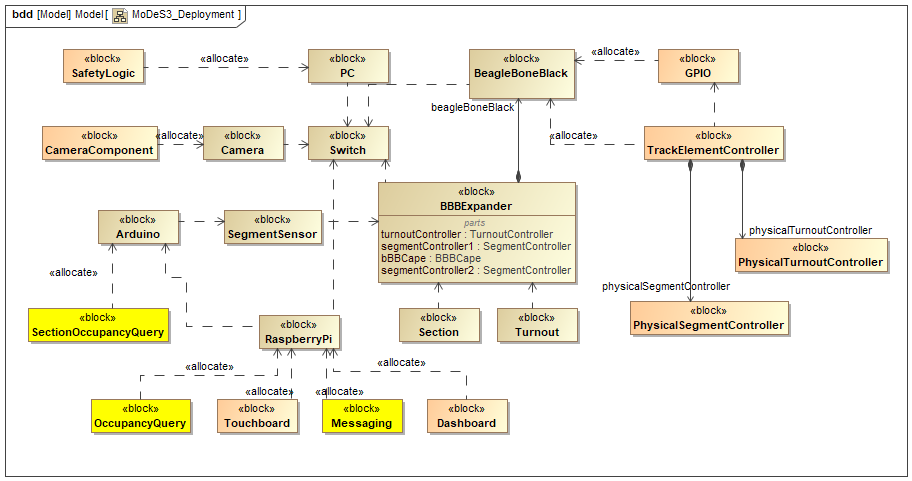
\includegraphics[width=150mm, keepaspectratio]{figures/testDesign/testLayoutSYSML/MoDeS3_Deployment-test1.png}
%	\caption{Integration test layout 1}
%	\label{fig:MoDeS3_Deployment-test1}
%\end{figure}
%
%\paragraph{Integration test layout 2}
%Aim of this test is to verify the software components, which is deployed to the \textit{BBB} and responsible for controlling the physical segments (see \ref{par:FunctionTEC} section for more description about this function). All the 6 \textit{BBB} have separate instance of \textbf{Track Element Controller} software function. This component gets an information through the network on command topics (shown in \ref{par:MQTTTopicCommand} section), when segment allowance or turnout state must be changed. At this point the control differentiates into subcomponents weather a turnout or a section command have been received. After command execution the \textit{Track Element Controller} sends the new status on the \textit{status topic} (see \ref{par:MQTTTopicStatus}). Both branches uses GPIO software component for giving impulse on the BBB cape pins.
%\begin{figure}[!h]
%	\centering
%	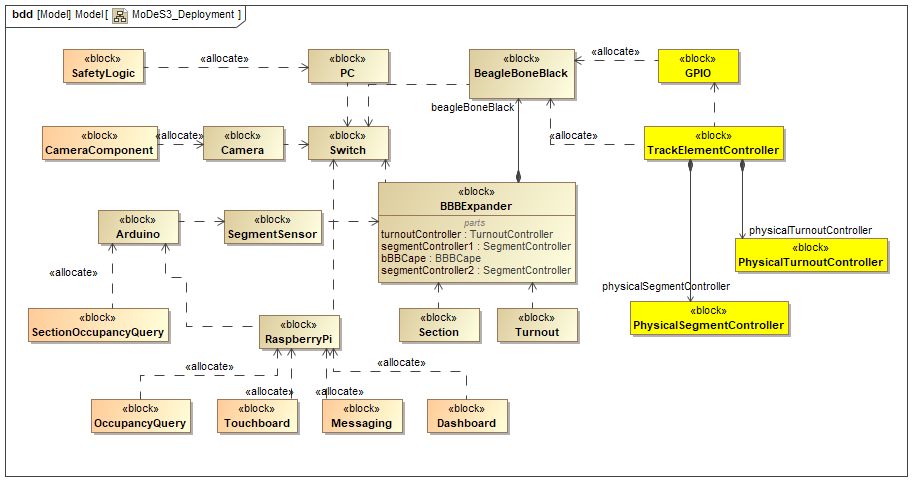
\includegraphics[width=150mm, keepaspectratio]{figures/testDesign/testLayoutSYSML/MoDeS3_Deployment-test2.png}
%	\caption{Integration test layout 2}
%	\label{fig:MoDeS3_Deployment-test2}
%\end{figure}
%
%\paragraph{Integration test layout 3}
%In this integration test we want to verify the decisions of \textit{Safety Logic} component. After we have verified the \textit{Safety Logic} as a unit and the occupancy detection elements, we can investigate the \textit{Safety Logic} decision based on the generated occupancy states together. These signs can be injected into the \textit{Arduino} hardware element or into the Section Occupancy Query directly.
%\begin{figure}[!h]
%	\centering
%	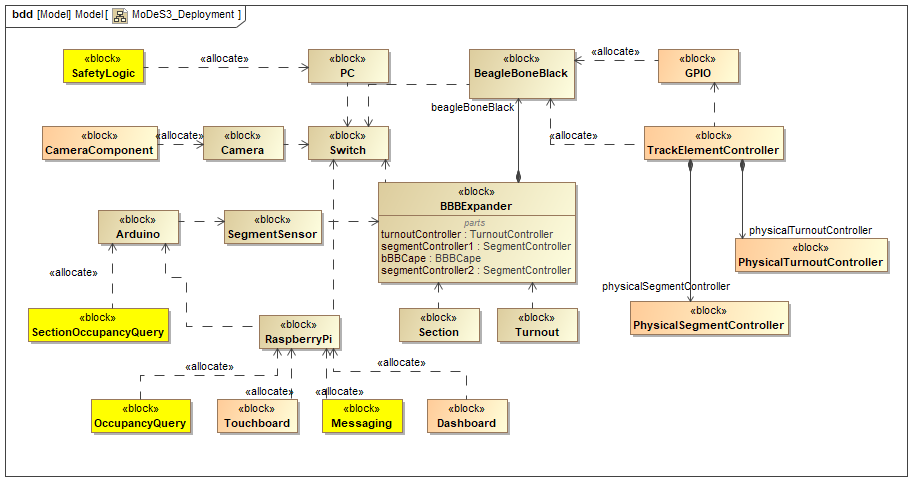
\includegraphics[width=150mm, keepaspectratio]{figures/testDesign/testLayoutSYSML/MoDeS3_Deployment-test3.png}
%	\caption{Integration test layout 3}
%	\label{fig:MoDeS3_Deployment-test3}
%\end{figure}
%
%\paragraph{Integration test layout 4}
%The fourth integration test should be a verification of an action after a \textit{Safety Logic} decision. In details, we can inject a critical scenario into the \textit{Safety Logic} component where a safety intervention needed and check the GPIO component's file writing operations.
%\begin{figure}[!h]
%	\centering
%	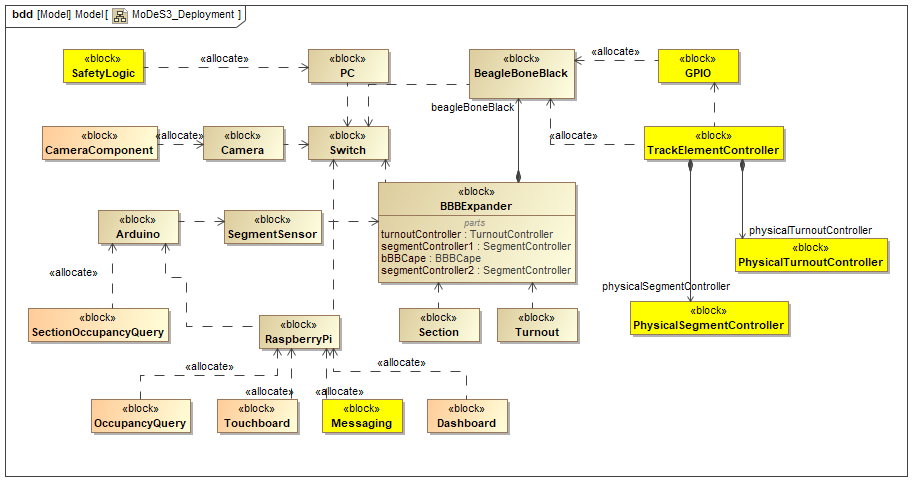
\includegraphics[width=150mm, keepaspectratio]{figures/testDesign/testLayoutSYSML/MoDeS3_Deployment-test4.png}
%	\caption{Integration test layout 4}
%	\label{fig:MoDeS3_Deployment-test4}
%\end{figure}
%
%\todo[inline]{Extend test cases}
%
%\subsection{System test}
%In the system tests all components are involved and only the injected, specific scenario is different. 
%I have already mentioned a few collision scenario in \ref{par:trainScenarios} section, and I just want to add three more scenarios with the double-turnout. First of them (see figure \ref{fig:LayoutT3-scenario1}) is a typical case, where the collision can be easily avoided with \textit{Train 1} waiting.
%\begin{figure}[!h]
%	\centering
%	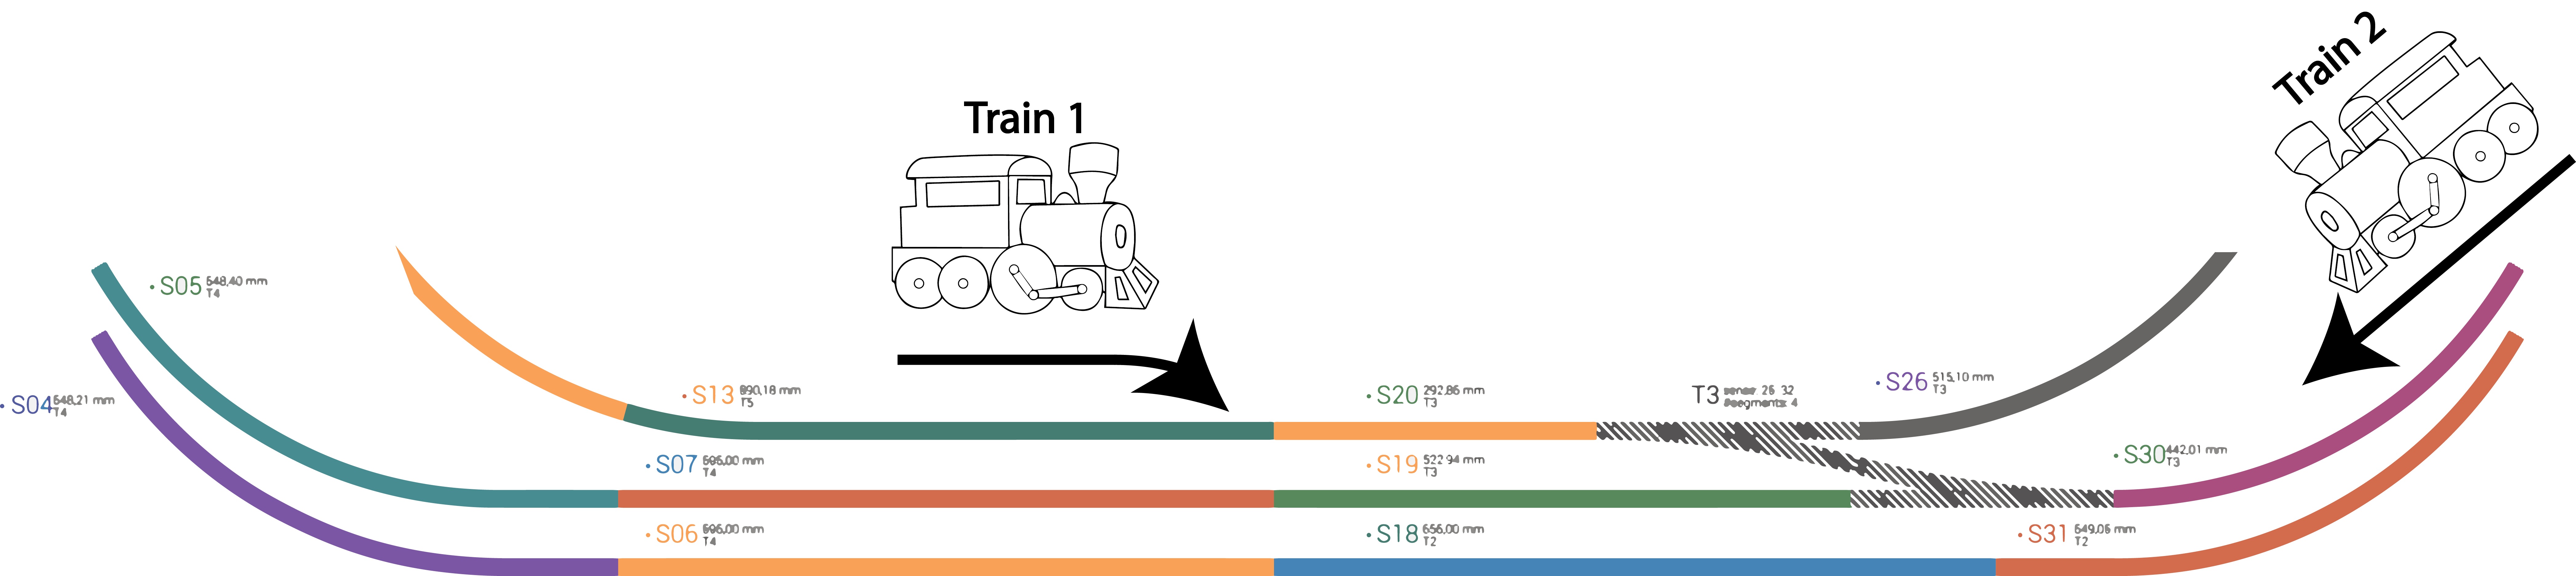
\includegraphics[width=150mm, keepaspectratio]{figures/modes3/layoutT3-scenario1.png}
%	\caption{Turnout 3 collision scenario 1}
%	\label{fig:LayoutT3-scenario1}
%\end{figure}
%
%The next possible collision could happen, when our two trains going exactly into each other after 2 sections.
%\begin{figure}[!h]
%	\centering
%	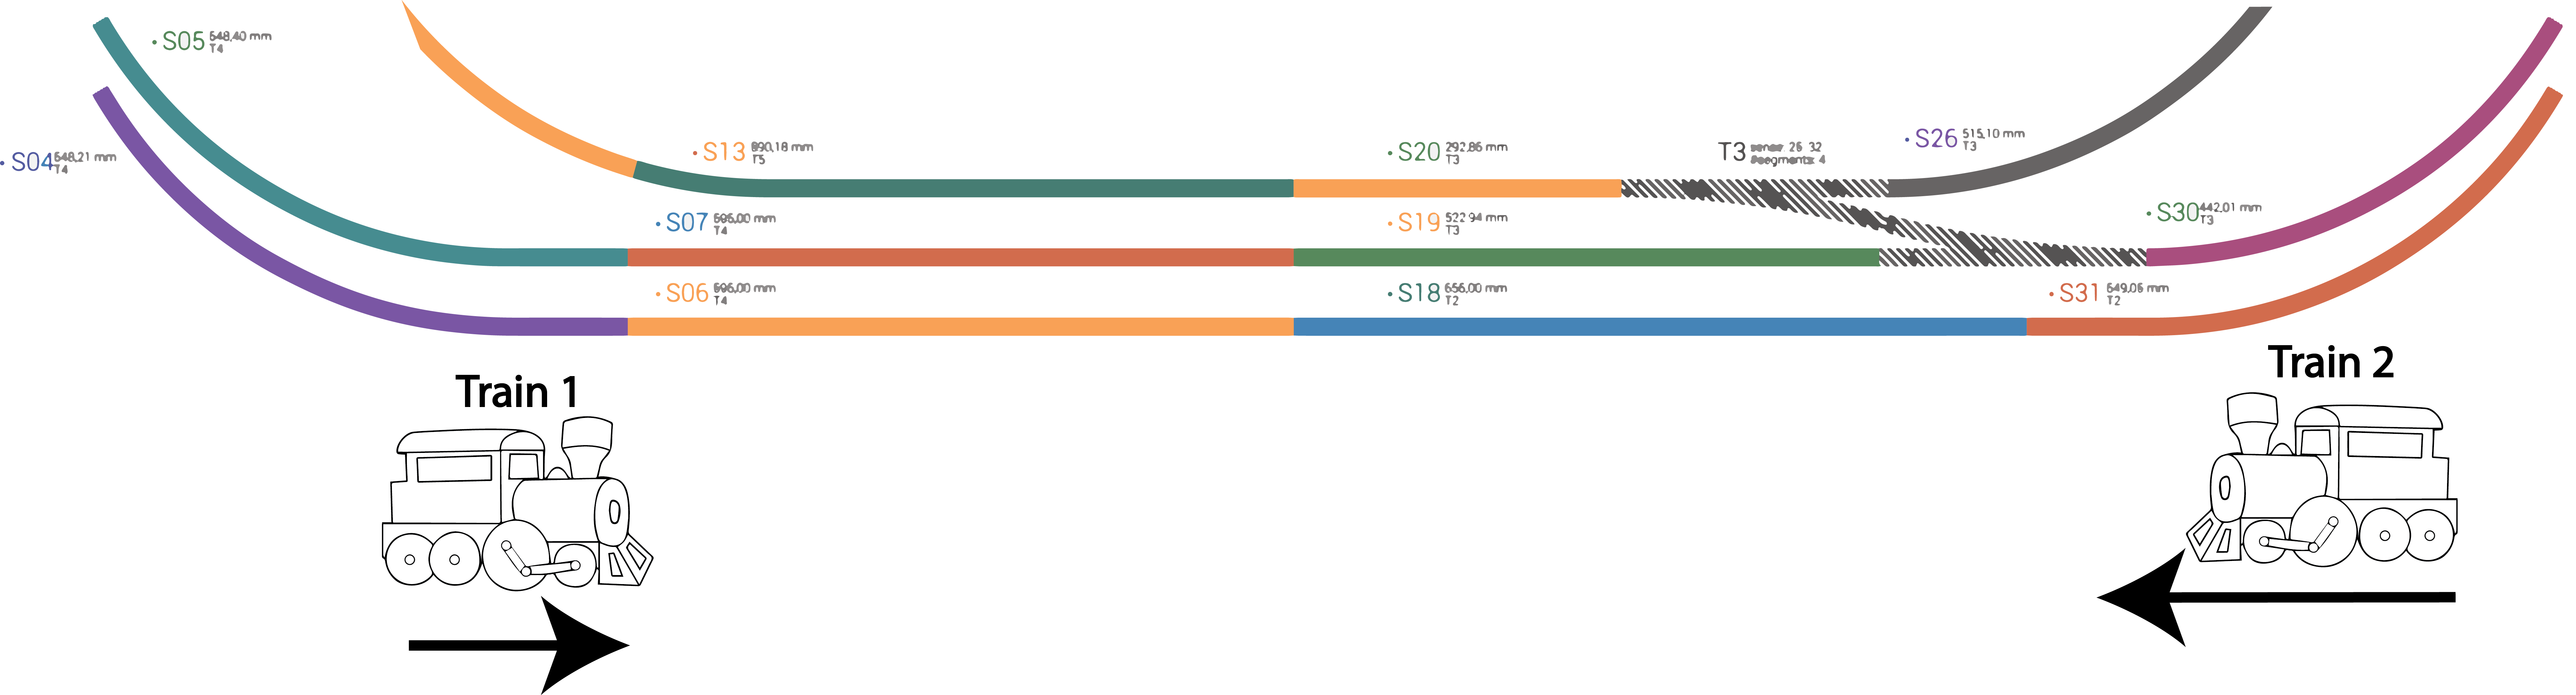
\includegraphics[width=150mm, keepaspectratio]{figures/modes3/layoutT3-scenario2.png}
%	\caption{Turnout 3 collision scenario 2}
%	\label{fig:LayoutT3-scenario2}
%\end{figure}
%\todo[inline]{Only With the bottom track its more understandable}
%
%The third scenario is similar with the first one, but if our T3 turnout is in a right direction (both turnout is in the straight direction), our trains are safe.
%\begin{figure}[!h]
%	\centering
%	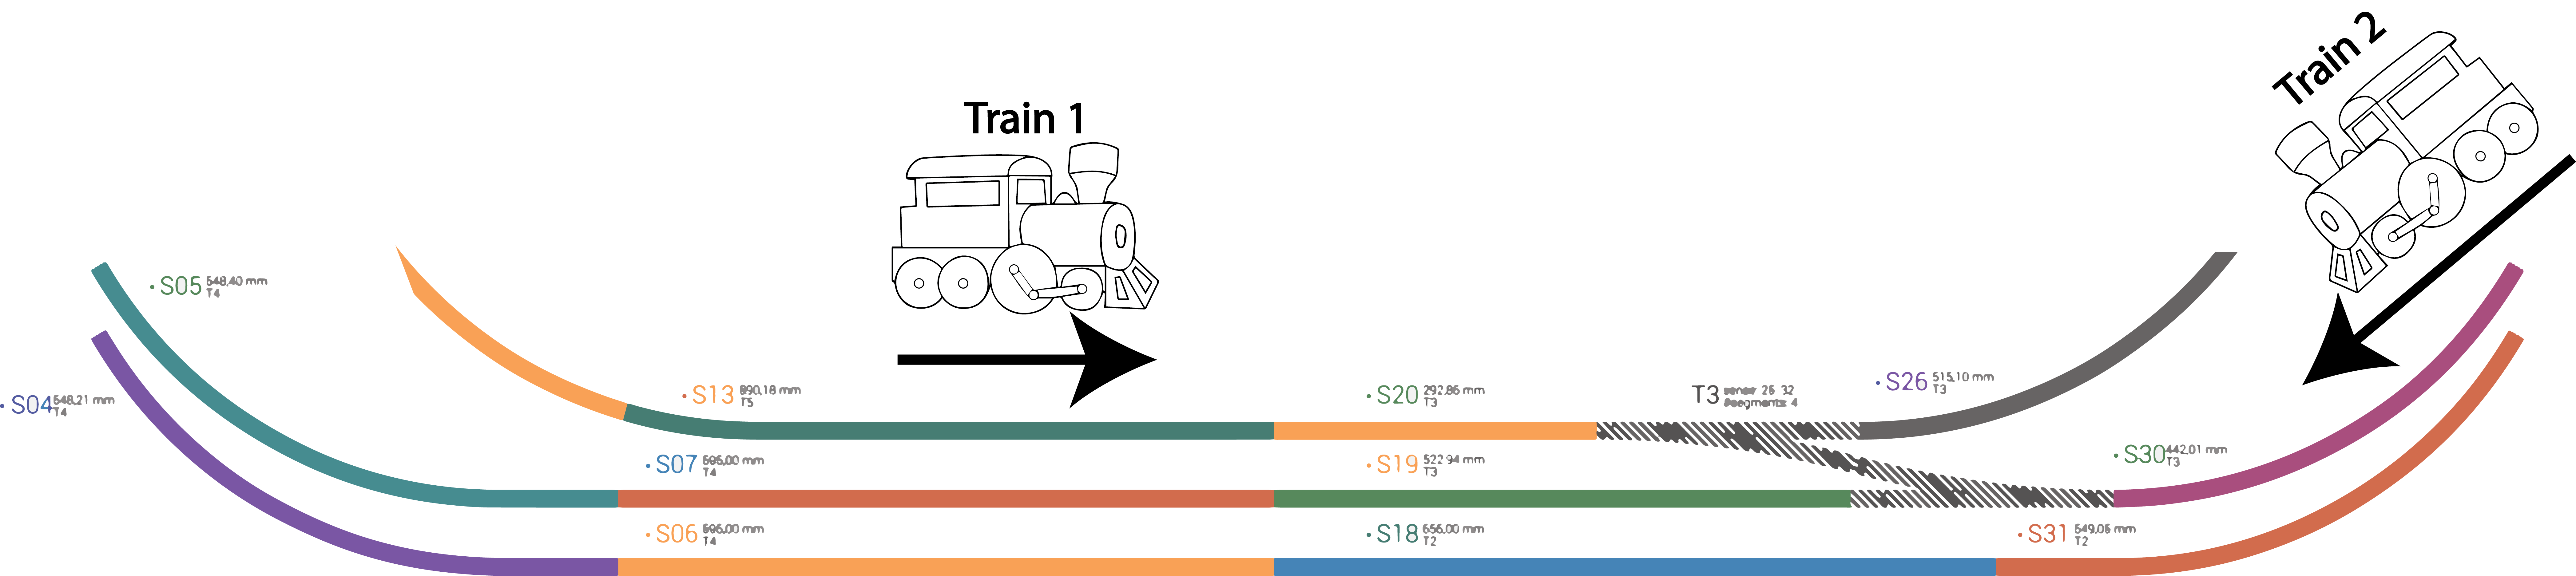
\includegraphics[width=150mm, keepaspectratio]{figures/modes3/layoutT3-scenario3.png}
%	\caption{Turnout 3 collision scenario 3}
%	\label{fig:LayoutT3-scenario3}
%\end{figure}